% CVPR 2023 Paper Template
% based on the CVPR template provided by Ming-Ming Cheng (https://github.com/MCG-NKU/CVPR_Template)
% modified and extended by Stefan Roth (stefan.roth@NOSPAMtu-darmstadt.de)

\documentclass[10pt,twocolumn,letterpaper]{article}

%%%%%%%%% PAPER TYPE  - PLEASE UPDATE FOR FINAL VERSION
% \usepackage[review]{cvpr}      % To produce the REVIEW version
% \usepackage{cvpr}              % To produce the CAMERA-READY version
\usepackage[pagenumbers]{cvpr} % To force page numbers, e.g. for an arXiv version

% Include other packages here, before hyperref.
\usepackage{graphicx}
\usepackage{amsmath}
\usepackage{amssymb}
\usepackage{booktabs}


% It is strongly recommended to use hyperref, especially for the review version.
% hyperref with option pagebackref eases the reviewers' job.
% Please disable hyperref *only* if you encounter grave issues, e.g. with the
% file validation for the camera-ready version.
%
% If you comment hyperref and then uncomment it, you should delete
% ReviewTempalte.aux before re-running LaTeX.
% (Or just hit 'q' on the first LaTeX run, let it finish, and you
%  should be clear).
\usepackage[pagebackref,breaklinks,colorlinks]{hyperref}


% Support for easy cross-referencing
\usepackage[capitalize]{cleveref}
\crefname{section}{Sec.}{Secs.}
\Crefname{section}{Section}{Sections}
\Crefname{table}{Table}{Tables}
\crefname{table}{Tab.}{Tabs.}


%%%%%%%%% PAPER ID  - PLEASE UPDATE
\def\cvprPaperID{*****} % *** Enter the CVPR Paper ID here
\def\confName{CVPR}
\def\confYear{2023}


\begin{document}

%%%%%%%%% TITLE - PLEASE UPDATE
\title{Suggestion for NLDL Winter School 2023}

\author{Anders Sildnes\\
University of Tromsø\\
Postboks 6050 Langnes\\
{\tt\small anders.sildnes@uit.no}
}
\maketitle

%%%%%%%%% ABSTRACT
% \begin{abstract}
% 
% \end{abstract}

%%%%%%%%% BODY TEXT
\section{Suggestion}
\label{sec:intro}
% Computational pathology is study of disease using methods such as artificial intelligence. For building models, there are three main hindrances: 1) lack of publicly available data, 2) large image-size and high number of details and 3) lack of ground truth data due to expert disagreeance. Consequently, developers have to compromise when building a model. To know if models are accurate enough, explainable AI can help. But, are the explanations good enough that a pathologist can trust a model used to evaluate patient diagnosis and/or prognosis? 

\cite{sslUMAP} uses self-supervised learning to learn morphological features of Lung Squamous Cell Carcinoma (LSCC). In training they use public TCGA and CPTAC datasets of H\&E-stained biopsy slides. They observe from previous work that other training algorithms cluster together tiles from the same slides, creating a batch effect where the algorithm learns features that are more slide specific than feature specific. This indicates that the network might do poorly on generalized input. They visualize this using 2D UMAP, shown in~\cref{fig:umap}.

\begin{figure}
  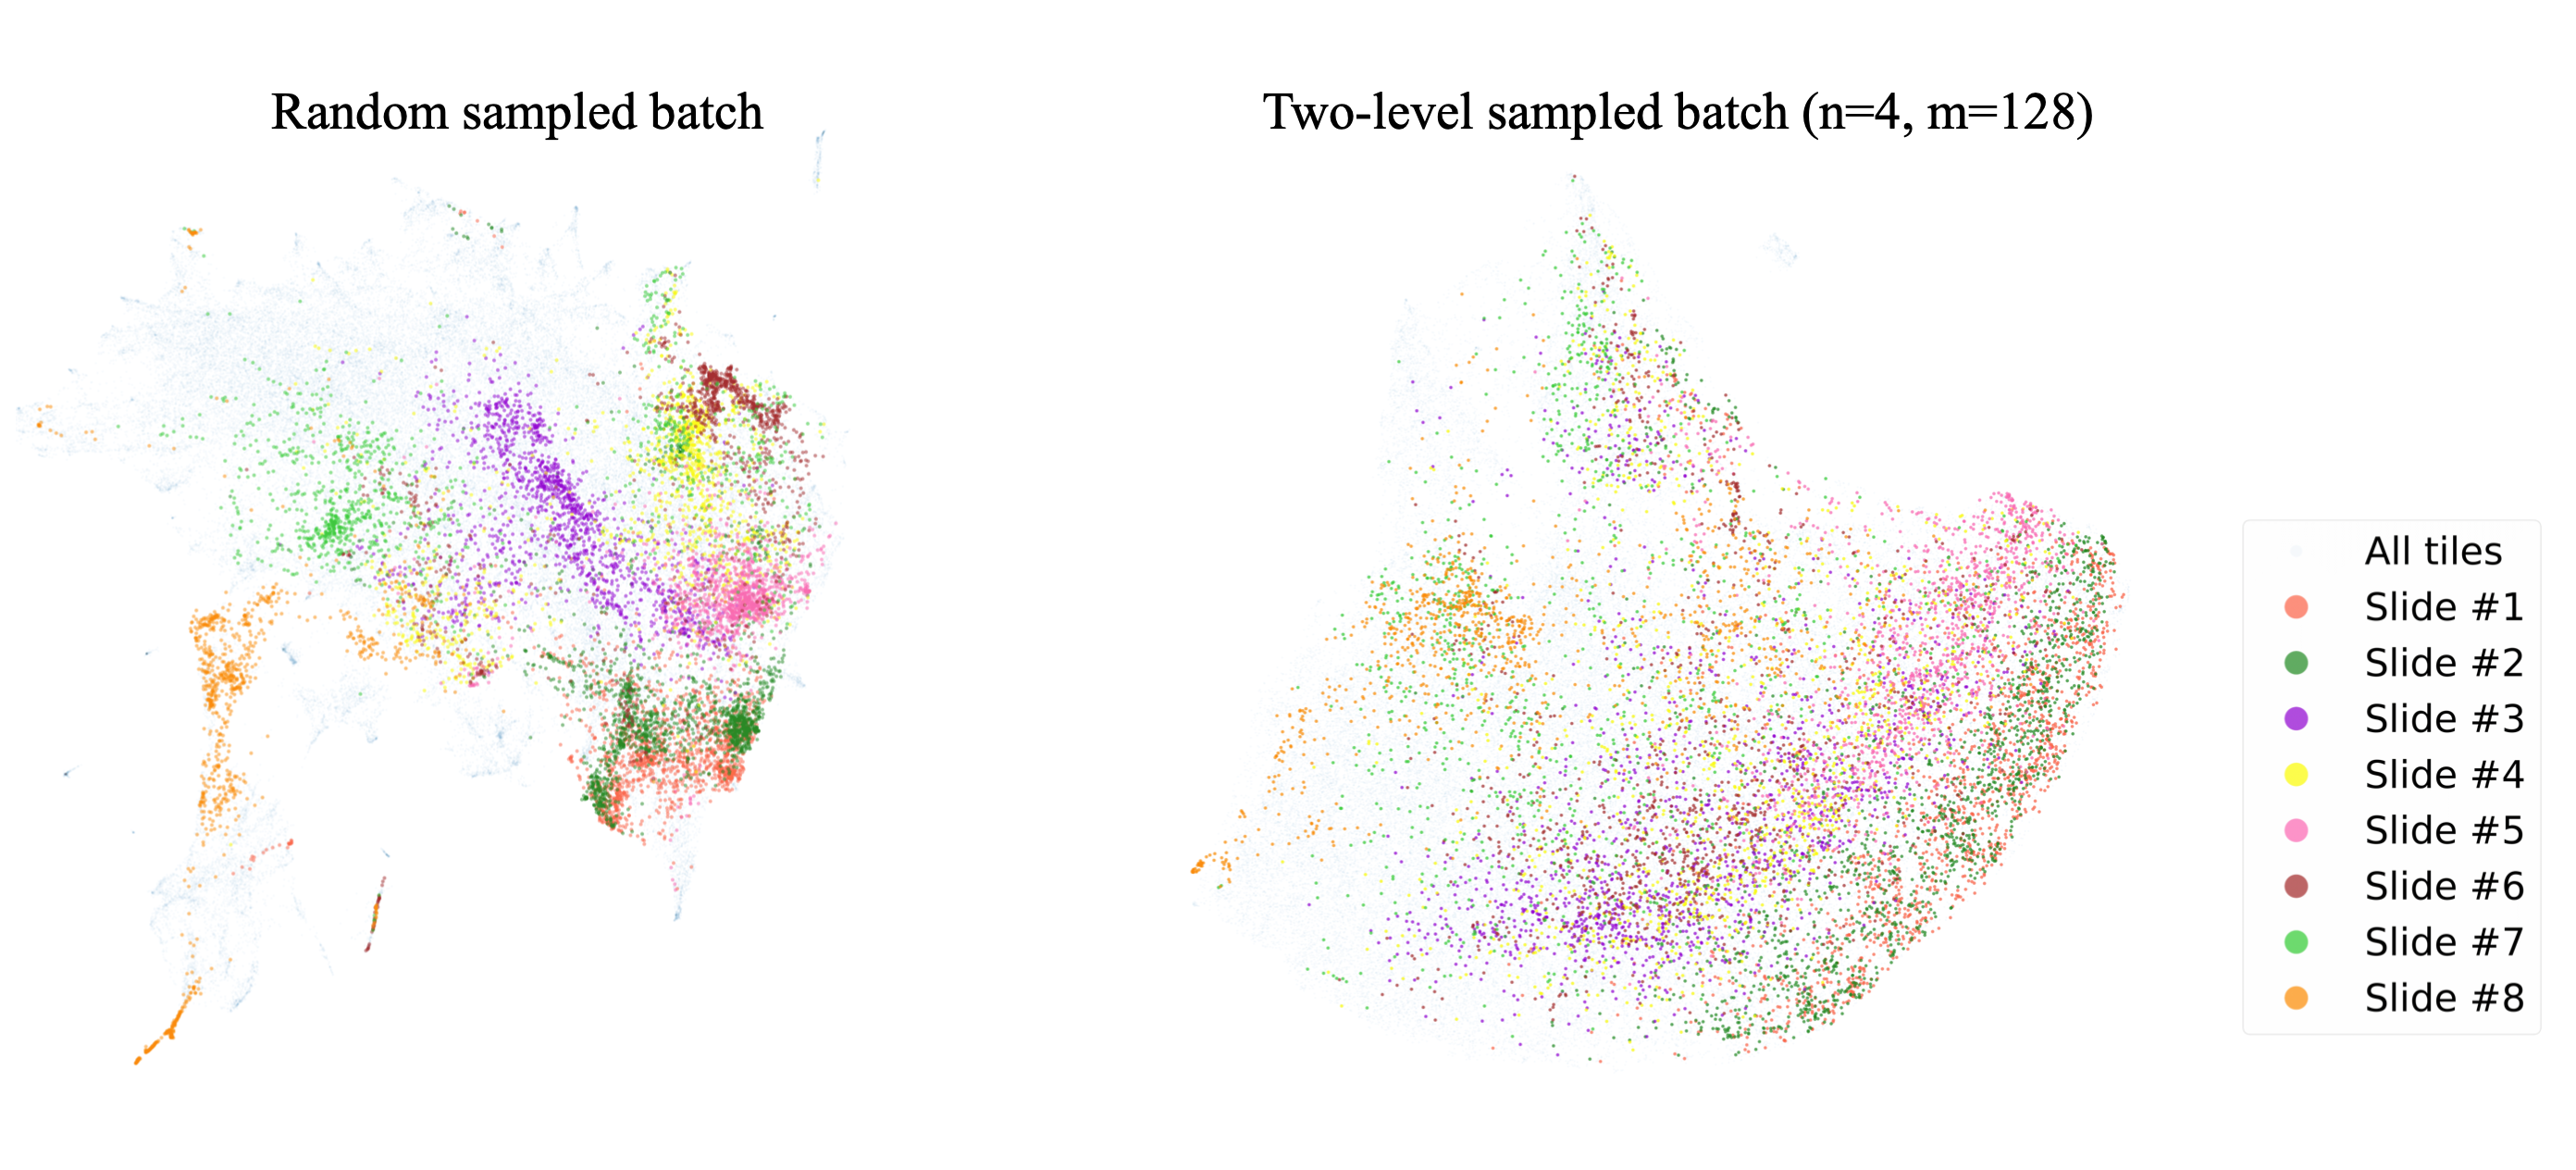
\includegraphics[scale=.17]{./umap.png}
  \caption{Figure taken entirely from~\cite{sslUMAP}. Both pictures show a 2D UMAP projection of tile representations. On the left a training algorithm with randomly sampled tiles from slides, showing that features learned in the same slide cluster together. Using a different sampling algorithm, the picture on the right shows a more even distribution w.r.t slides}
  \label{fig:umap}
\end{figure}

\subsection{UMAP}
 The algorithm is founded on three assumptions about the data
 \begin{enumerate}
    The data is uniformly distributed on Riemannian manifold;
    The Riemannian metric is locally constant (or can be approximated as such);
    The manifold is locally connected.
 \end{enumerate}


I wish to evaluate~\cite{sslUMAP} and quantify the quality of \textit{the explanation} using metrics inspired by Quantus~\cite{hedstrom2022quantus}. This means 1) finding relevant qualitative metrics for the given batch effect plots and 2) testing how the metrics change with model, batch and image adjustments. In particular, I am curious how well the metrics show batch/clustering effects for few (1-3) slides. This can be a useful indication early during a training process.

%%%%%%%%% REFERENCES
{\small
\bibliographystyle{ieee_fullname}
\bibliography{egbib}
}

\end{document}
